
\chapter{Kinetic Approach}











\section{Derivation of the Rate Equations}

We now treat the problem from the point of view of it's time evolution, and 
look at the results as $t \to \infty$ (see \cite{krapivsky1992kinetics}). We 
assume a line of fixed length $L$ with $L \to \infty$. We are interested in 
the distribution of gaps, the expected total gap length, and consequently 
the car coverage. Let $X_t$ be a random variable that represents the length 
of a gap at time $t$, with $N(x, t)$ the number of gaps less than or equal 
to $x$, and $N(t)$ the total number of gaps. We define the gap length 
distribution $F(x, t)$ as follows: \bigskip

\[
	P(X_t \leq x) = F(x, t) = \frac{N(x, t)}{N(t)}
\]\medskip

here $P(A)$ represents the probability of event $A$ occurring. The gap length 
density function $f(x, t)$ is then: \bigskip

\begin{eqnarray} \label{eq:10}
	f(x, t) = \frac{\partial F}{\partial x} = \frac{1}{N(t)} \frac{\partial N}{\partial x} (x, t)
\end{eqnarray}\medskip

therefore the probability that a gap has length between $a$ and $b$ is: \bigskip

\[
	\int_{a}^{b} f(x, t) dx = \frac{1}{N(t)} \int_{a}^{b} \frac{\partial N}{\partial x} (x, t) dx
\]\medskip

which is simply the number of gaps with length between $a$ and $b$ divided by 
the total number of gaps at time $t$. We define the coverage function, 
$\theta(t)$, the proportion of $L$ occupied by cars as: \bigskip

\[
	\theta(t) = \frac{N(t)}{L}
\]\medskip

i.e. the total number of gaps, which is also the total number of cars of unit 
length, divided by the line length. We define the expectation of $X_t$, the 
average length of a gap, as: \bigskip

\[
	E(X_t) = \int_{0}^{\infty} x f(x, t) dx
\]\medskip

We now define the gap density function, $P(x, t)$, as: \bigskip

\begin{eqnarray} \label{eq:11}
	P(x, t) = \frac{1}{L} \frac{\partial N}{\partial x} (x, t)
\end{eqnarray}\medskip

where $L$ is the length of the line. Therefore the proportion of gaps with length between 
$a$ and $b$ is: \bigskip

\[
	\int_{a}^{b} P(x, t) dx = \frac{1}{L} \int_{a}^{b} \frac{\partial N}{\partial x} (x, t) dx
\]\medskip

combining equations \ref{eq:10} and \ref{eq:11} above we have: \bigskip

\[
	f(x, t) = \frac{L \cdot P(x, t)}{N(t)}
\]\medskip

from which we get an expression, in terms of $P(x, t)$, for the expected total gap length 
at time $t$: \bigskip

\begin{eqnarray*}
	N(t) \cdot E(X_t) & = & N(t) \int_{0}^{\infty} x f(x, t) dx \\\\
					  & = & L \int_{0}^{\infty} x P(x, t) dx
\end{eqnarray*}\medskip

which is the expected total gap length at time $t$. Returning to the coverage function 
$\theta(t)$, we now express it in terms of the above expected total gap length by observing 
that: \bigskip

\[
	\theta(t) = 1 - \frac{N(t) \cdot E(X_t)}{L}
\]\medskip

from which we get: \bigskip

\[
	\theta(t) = 1 - \int_{0}^{\infty} x P(x, t) dx
\]\medskip

and noting that the sum pf all gap lengths and car lengths gives us the total line length 
$L$, we find a new expression for $\theta(t)$: \bigskip

\begin{eqnarray*}
									 L & = & L \int_{0}^{\infty} (x + 1) P(x, t) dx \\\\
									 1 & = & \int_{0}^{\infty} (x + 1) P(x, t) dx \\\\
									   & = & \int_{0}^{\infty} x P(x, t) dx + \int_{0}^{\infty} P(x, t) dx \\\\
	1 - \int_{0}^{\infty} x P(x, t) dx & = & \int_{0}^{\infty} P(x, t) dx
\end{eqnarray*}\medskip

from which we see that: \bigskip

\[
	\theta(t) = \int_{0}^{\infty} P(x, t) dx
\]\medskip

Returning to our gap density function, $P(x, t)$, we form a rate equation using our 
expressions for the gap density function: \bigskip

\begin{eqnarray*}
	\frac{\partial P(x, t)}{\partial t} = 
	\begin{dcases}
		2 \int_{x + 1}^{\infty} P(y, t) dy                     & \text{for } x < 1 \\\\
		-(x - 1) P(x, t) + 2 \int_{x + 1}^{\infty} P(y, t) dy  & \text{for } x \geq 1
	\end{dcases}
\end{eqnarray*}\medskip

which is composed of creation and destruction terms. The creation term may be be 
understood by considering a gap of length $y \geq x + 1$, there are exactly two 
ways to park within this gap that will result in a gap of length $x$. The 
destruction term, which only appears in the case where $x \geq 1$, deals with 
the case where an existing gap of length $x$ is destroyed by parking a car within 
it - in this case the remaining length becomes $x - 1$, and this destruction can be 
accomplished in $P(x, t)$ ways. \bigskip










\section{Solving the Rate Equations}

We will now solve the rate equation using the following two initial conditions: \bigskip

\[
	P(x, 0) = 0 \quad \forall x
\]\medskip

and: \bigskip

\[
	\lim_{t \to 0} \int_{0}^{\infty} x P(x, t) dx = 1
\]\medskip

We make the following substitution: \bigskip

\[
	P(x, t) = A(t) e^{-(x - 1)t}
\]\medskip

and begin by looking at our initial conditions. The first becomes: \bigskip

\begin{eqnarray*}
	P(x, 0) & = & A(0) e^0 \\
			& = & A(0) \\
			& = & 0
\end{eqnarray*}\medskip

and the second becomes: \bigskip

\begin{eqnarray*}
	\lim_{t \to 0} \int_{0}^{\infty} x P(x, t) dx & = & \lim_{t \to 0} \int_{0}^{\infty} x A(t) e^{-(x - 1)t} dx \\\\
												  & = & \lim_{t \to 0} A(t) \int_{0}^{\infty} x e^{-(x - 1)t} dx 
\end{eqnarray*}\medskip

integrating by parts we get: \bigskip

\begin{eqnarray*}
	\int_{0}^{\infty} x e^{-(x - 1)t} dx & = & \left. \frac{x e^{-(x - 1)t}}{-t} \right|_{x = 0}^{\infty} - \int_{0}^{\infty} \frac{e^{-(x - 1)t}}{-t} dx \\\\
										 & = & \left. \frac{e^{-(x - 1)t}}{-t^2} \right|_{x = 0}^{\infty} \\\\
										 & = & \frac{e^t}{t^2}
\end{eqnarray*}\medskip

and putting the result into the above gives us: \bigskip

\begin{eqnarray*}
	\lim_{t \to 0} A(t) \int_{0}^{\infty} x e^{-(x - 1)t} dx & = & 1 \\\\
						 \lim_{t \to 0} \frac{A(t) e^t}{t^2} & = & 1 \\\\
			\therefore \quad \lim_{t \to 0} \frac{A(t)}{t^2} & = & 1
\end{eqnarray*}\medskip

For $x \geq 1$: \bigskip

\begin{eqnarray*}
			\frac{\partial}{\partial t} (A(t) e^{-(x - 1)t}) & = & -(x - 1) A(t) e^{-(x - 1)t} + 2 \int_{x + 1}^{\infty} A(t) e^{-(y - 1)t} dy \\\\
	A^{\prime}(t) e^{-(x - 1)t} - (x - 1) A(t) e^{-(x - 1)t} & = & -(x - 1) A(t) e^{-(x - 1)t} + 2 A(t) \left. \frac{e^{-(y - 1)t}}{-t} \right|_{y = x + 1}^{\infty} \\\\
								 A^{\prime}(t) e^{-(x - 1)t} & = & 2 A(t) \frac{e^{-t}}{t} e^{-(x - 1)t} \\\\
 											   A^{\prime}(t) & = & 2 A(t) \frac{e^{-t}}{t}  
\end{eqnarray*}\medskip

which is an ODE. If we make a further substitution $A(t) = t^2 F(t)$ our initial condition becomes: \bigskip

\begin{eqnarray*}
		\lim_{t \to 0} \frac{A(t)}{t^2} & = & 1 \\\\
	\lim_{t \to 0} \frac{t^2 F(t)}{t^2} & = & 1 \\\\
					\lim_{t \to 0} F(t) & = & 1 \\\\
								   F(0) & = & 1 
\end{eqnarray*}\medskip

and our equation becomes: \bigskip

\begin{eqnarray*}
												   A^{\prime}(t) & = & 2 A(t) \frac{e^{-t}}{t} \\\\
									2 t F(t) + t^2 F^{\prime}(t) & = & 2 t F(t) e^{-t} \\\\
										2 F(t) + t F^{\prime}(t) & = & 2 F(t) e^{-t} \\\\
												 t F^{\prime}(t) & = & 2 F(t) e^{-t} - 2 F(t) \\\\
																 & = & F(t) \left( 2 ( e^{-t} - 1 ) \right) \\\\
							 					   F^{\prime}(t) & = & F(t) \left( 2 \frac{(e^{-t} - 1)}{t} \right) \\\\
	F^{\prime}(t) + F(t) \left( 2 \frac{(1 - e^{-t})}{t} \right) & = & 0 
\end{eqnarray*}\medskip

we solve this using the integrating factor: \bigskip

\[
	I(t) = \exp \left( 2 \int_{0}^{t} \frac{(1 - e^{-\tau})}{\tau} d\tau \right)
\]\medskip

which gives us: \bigskip

\begin{eqnarray*}
	F^{\prime}(t) \cdot I(t) + F(t) \cdot I(t) \left( 2 \frac{(1 - e^{-t})}{t} \right) & = & 0 \\\\
								   F^{\prime}(t) \cdot I(t) + F(t) \cdot I^{\prime}(t) & = & 0 \\\\
														\frac{d}{dt} (F(t) \cdot I(t)) & = & 0 \\\\
												  					   F(t) \cdot I(t) & = & C \\\\
												  								  F(t) & = & \frac{C}{I(t)}
\end{eqnarray*}\medskip

we make use of our initial condition $F(0) = 1$ and the fact that $I(0) = 1$ to find $C$: \bigskip

\begin{eqnarray*}
	F(0) & = & \frac{C}{I(0)} \\\\
	   C & = & 1 
\end{eqnarray*}\medskip

and hence: \bigskip

\[
	F(t) = \exp \left( -2 \int_{0}^{t} \frac{(1 - e^{-\tau})}{\tau} d\tau \right)
\]\medskip

And for $x < 1$: \bigskip

\begin{eqnarray*}
	\frac{\partial P(x, t)}{\partial t} & = & 2 \int_{x + 1}^{\infty} P(y, t) dy \\\\
										& = & 2 \int_{x + 1}^{\infty} t^2 F(t) e^{-(y - 1)t} dy \\\\
										& = & 2 t^2 F(t) \int_{x + 1}^{\infty} e^{-(y - 1)t} dy \\\\
										& = & 2 t^2 F(t) \left. \frac{e^{-(y - 1)t}}{-t} \right|_{y = x + 1}^{\infty} \\\\
										& = & 2 t F(t) \left. e^{-(y - 1)t} \right|_{y = x + 1}^{\infty} \\\\
										& = & 2 t F(t) e^{-xt} \\\\
			   \therefore \quad P(x, t) & = & 2 \int_{0}^{t} \tau F(\tau) e^{-x\tau} d\tau 
\end{eqnarray*}\medskip

So our gap density function can be expressed as follows: \bigskip

\begin{eqnarray*}
	P(x, t) = 
	\begin{dcases}
		2 \int_{0}^{t} \tau F(\tau) e^{-x\tau} d\tau		& \text{for } x < 1 \\\\
		t^2 F(t) e^{-(x - 1)t}								& \text{for } x \geq 1
	\end{dcases}
\end{eqnarray*}\medskip

with $F(t)$ as above. Returning to our coverage function, and making use of the above expression 
for the gap density function, we have: \bigskip

\[
	\theta(t) = \int_{0}^{1} \left( 2 \int_{0}^{t} \tau F(\tau) e^{-x\tau} d\tau \right) dx + \int_{1}^{\infty} t^2 F(t) e^{-(x - 1)t} dx \\\\
\]\medskip

Differentiating with respect to $t$ we get: \bigskip

\[
	\frac{d \theta}{dt} = \frac{\partial}{\partial t}  \int_{0}^{1} \left( 2 \int_{0}^{t} \tau F(\tau) e^{-x\tau} d\tau \right) dx + \frac{\partial}{\partial t}  \int_{1}^{\infty} t^2 F(t) e^{-(x - 1)t} dx 
\]\medskip

We will deal with each part of the right hand side separately. Starting with the first part: \bigskip

\begin{eqnarray*}
	\frac{\partial}{\partial t}  \int_{0}^{1} \left( 2 \int_{0}^{t} \tau F(\tau) e^{-x\tau} d\tau \right) dx & = & \int_{0}^{1} \left( 2 \frac{\partial}{\partial t}  \int_{0}^{t} \tau F(\tau) e^{-x\tau} d\tau \right) dx \\\\
																											 & = & \int_{0}^{1} \left( 2 t F(t) e^{-xt} \right) dx \\\\
																											 & = & 2 t F(t) \int_{0}^{1} e^{-xt} dx \\\\
																											 & = & 2 t F(t) \left. \frac{e^{-xt}}{-t} \right|_{x = 0}^{1} \\\\
																											 & = & 2 F(t) (1 - e^{-t}) 
\end{eqnarray*}\medskip

moving on to the second part: \bigskip

\begin{eqnarray*}
	\frac{\partial}{\partial t}  \int_{1}^{\infty} t^2 F(t) e^{-(x - 1)t} dx & = & \int_{1}^{\infty} \frac{\partial}{\partial t}  \left( t^2 F(t) e^{-(x - 1)t} \right) dx \\\\
																			 & = & \int_{1}^{\infty} \left( 2 t F(t) e^{-(x - 1)t} + t^2 F^{\prime}(t) e^{-(x - 1)t} + t^2 F(t) -(x - 1) e^{-(x - 1)t} \right) dx \\\\
																			 & = & \int_{1}^{\infty} 2 t F(t) e^{-(x - 1)t} dx \\\\
																			 &   & + \int_{1}^{\infty} t^2 F^{\prime}(t) e^{-(x - 1)t} dx \\\\
																			 &   & + \int_{1}^{\infty} t^2 F(t) -(x - 1) e^{-(x - 1)t} dx 
\end{eqnarray*}\medskip

taking each part of this integral separately: \bigskip

\begin{eqnarray*}
	\int_{1}^{\infty} 2 t F(t) e^{-(x - 1)t} dx & = & 2 t F(t) \int_{1}^{\infty} e^{-(x - 1)t} dx \\\\
												& = & 2 t F(t) \left. \frac{e^{-(x - 1)t}}{-t} \right|_{x = 1}^{\infty} \\\\
												& = & 2 F(t)
\end{eqnarray*}\medskip

followed by: \bigskip

\begin{eqnarray*}
	\int_{1}^{\infty} t^2 F^{\prime}(t) e^{-(x - 1)t} dx & = & t^2 F^{\prime}(t) \int_{1}^{\infty} e^{-(x - 1)t} dx \\\\
														 & = & t^2 F^{\prime}(t) \left. \frac{e^{-(x - 1)t}}{-t} \right|_{x = 1}^{\infty} \\\\
														 & = & t F^{\prime}(t) \\\\
														 & = & -2 F(t) (1 - e^{-t})
\end{eqnarray*}\medskip

here we have made use of the fact that: \bigskip

\[
	F^{\prime}(t) = -2 F(t) \frac{(1 - e^{-t})}{t}
\]\medskip

and: \bigskip

\begin{eqnarray*}
	\int_{1}^{\infty} t^2 F(t) -(x - 1) e^{-(x - 1)t} dx & = & t^2 F(t) \int_{1}^{\infty} -(x - 1) e^{-(x - 1)t} dx \\\\
														 & = & t^2 F(t) \left.  \frac{ x t e^{-(x - 1)t} - t e^{-(x - 1)t} + e^{-(x - 1)t} - 1 }{t^2}  \right|_{x = 1}^{\infty} \\\\
														 & = & -F(t) 
\end{eqnarray*}\medskip

finally putting it all together we get: \bigskip

\begin{eqnarray*}
		   \frac{d \theta}{dt} & = & 2 F(t) (1 - e^{-t}) + 2 F(t) - 2 F(t) (1 - e^{-t}) - F(t) \\\\
							   & = & F(t) \\\\
	\therefore \quad \theta(t) & = & \int_{0}^{t} F(\tau) d\tau
\end{eqnarray*}\medskip

We have derived an expression for the coverage function solely in terms of $t$, and in a 
very satisfying way. In figure \ref{fig:tcf1} we have used the above expression to plot 
the coverage function. As expected, $\theta(t)$ tends towards $C_R$, here denoted with a 
dashed red line. $C_R$ was calculated by evaluating $\theta(t)$ as $t \to \infty$. \bigskip

\begin{figure}[h!]
	\centering
	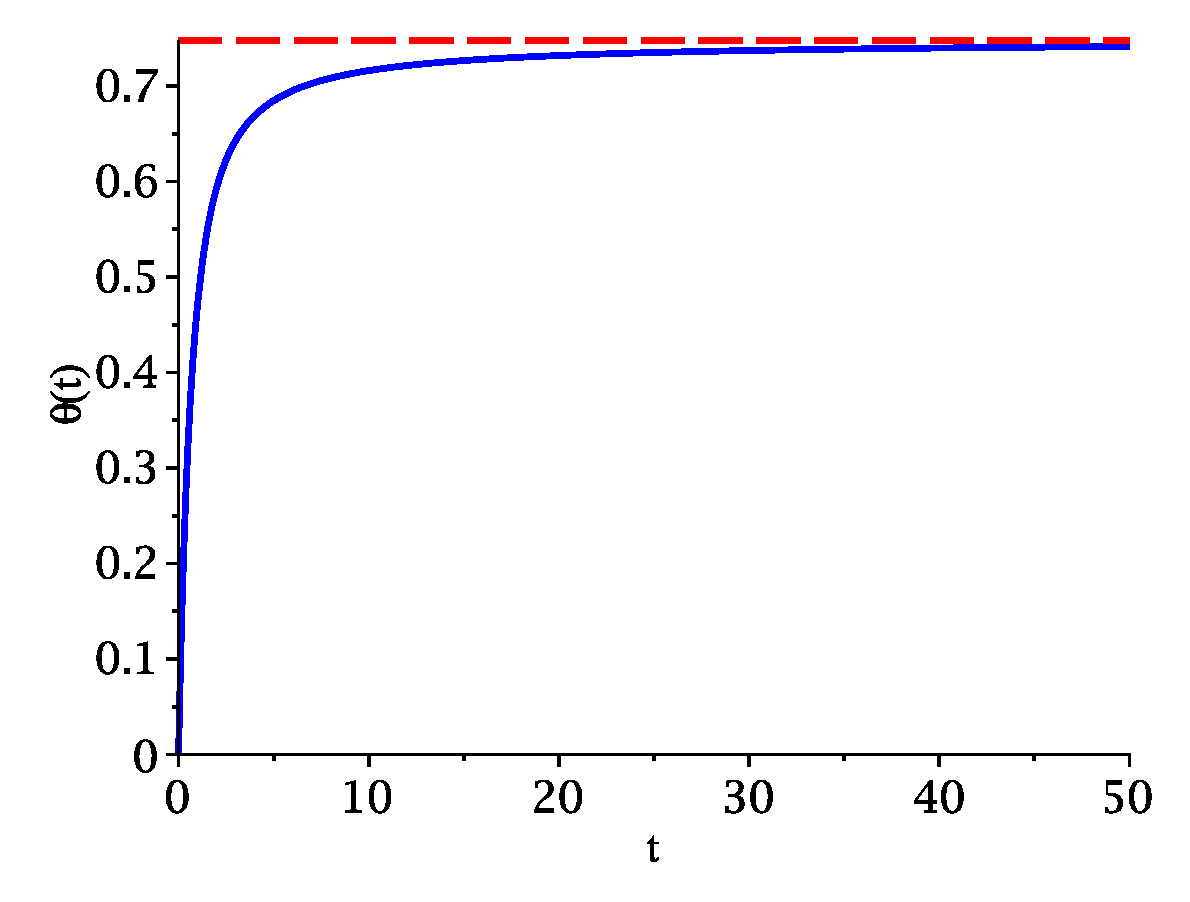
\includegraphics[scale = 0.35]{theta_01.eps}
%	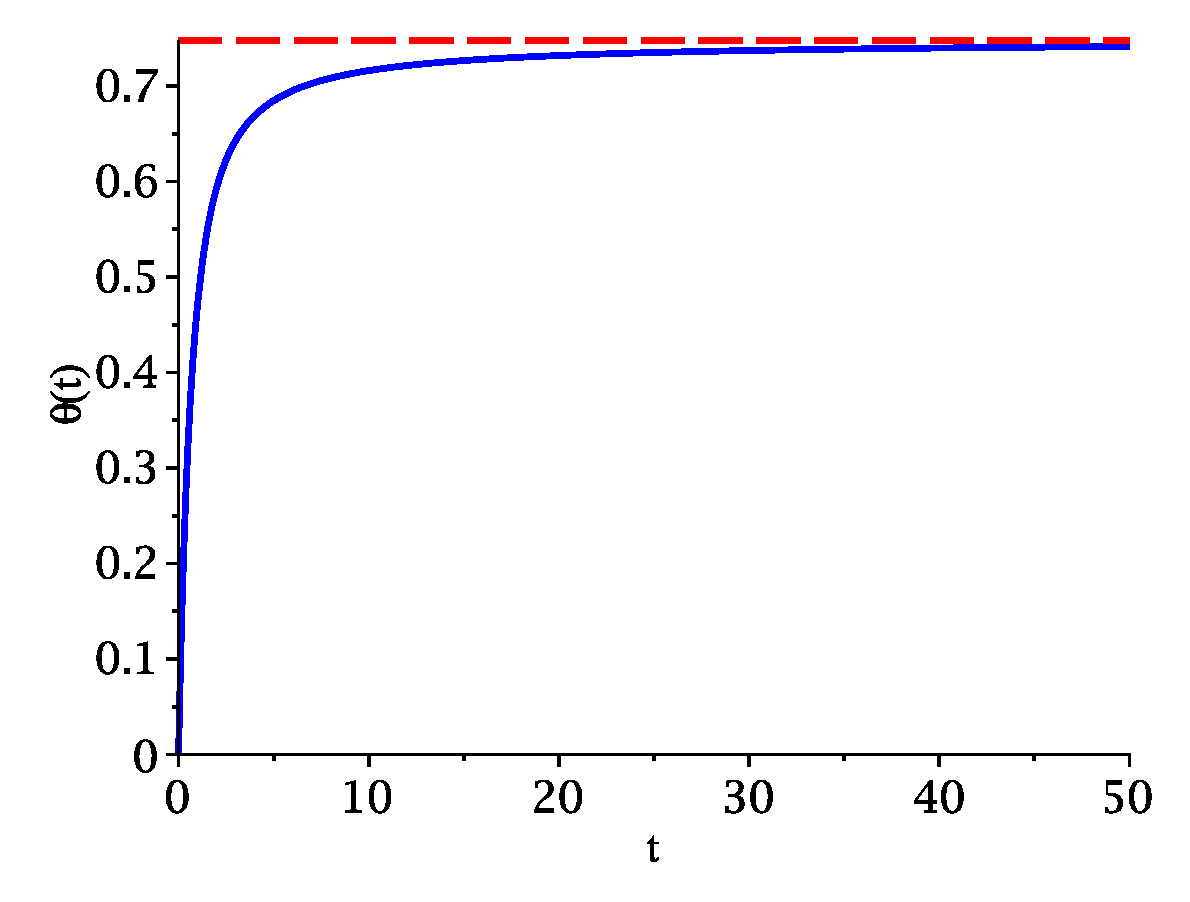
\includegraphics[width=\textwidth]{theta_01.eps}
	\caption{The coverage function}
	\label{fig:tcf1}
\end{figure}\medskip

We now look at the behaviour of the gap density function, $P(x, t)$, as a function of $x$ 
for different values of $t$. \bigskip

\begin{figure}[h!]
	\centering
%	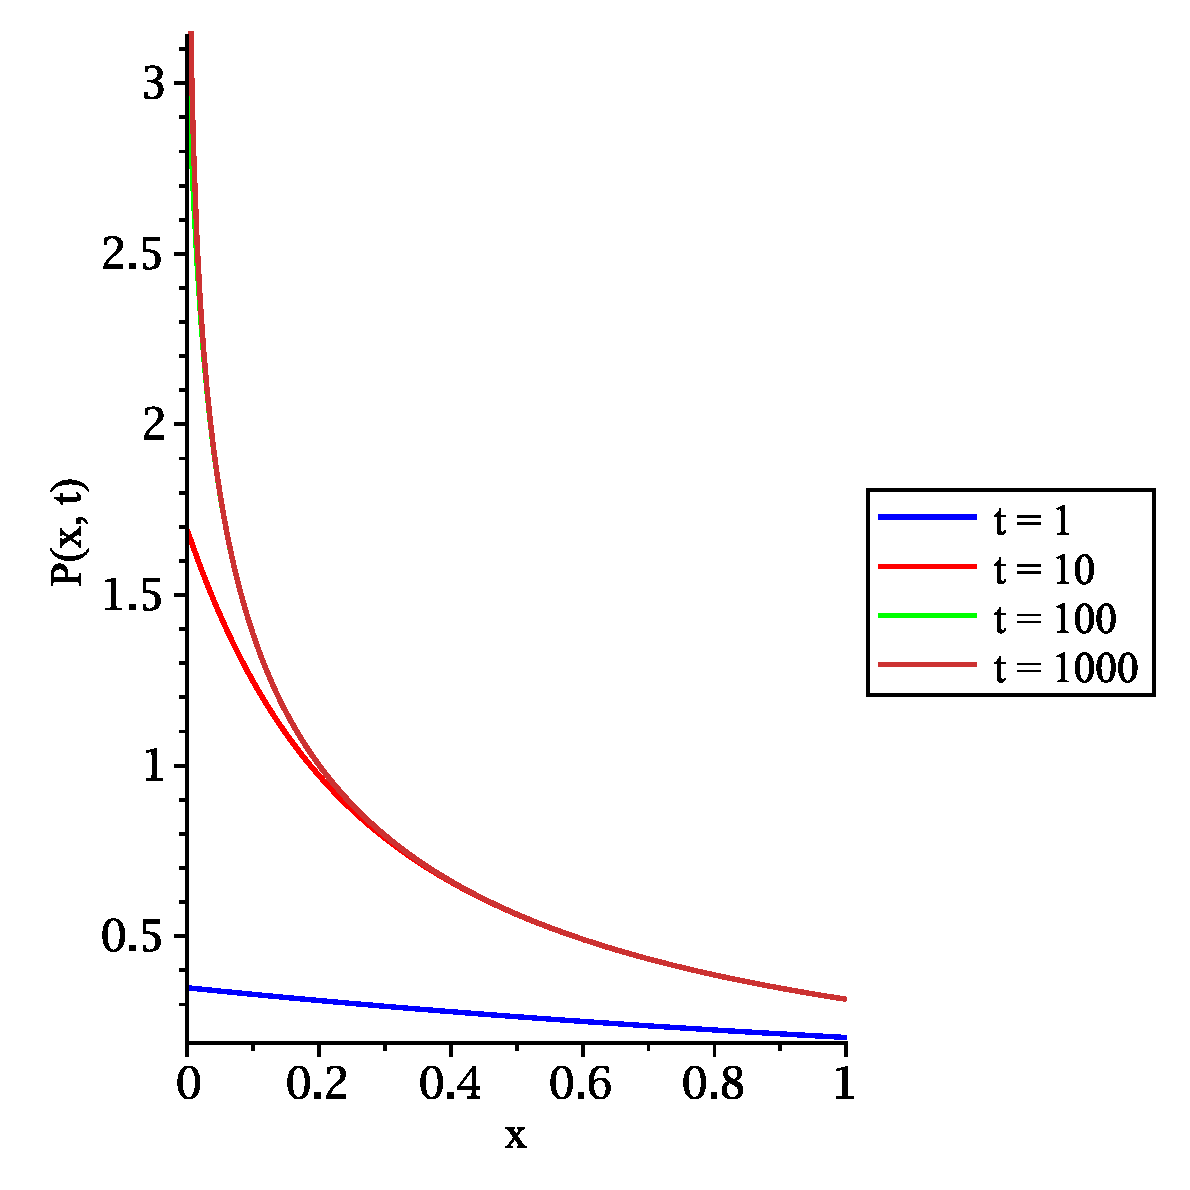
\includegraphics[scale = 0.35]{gap_density_01.eps}
	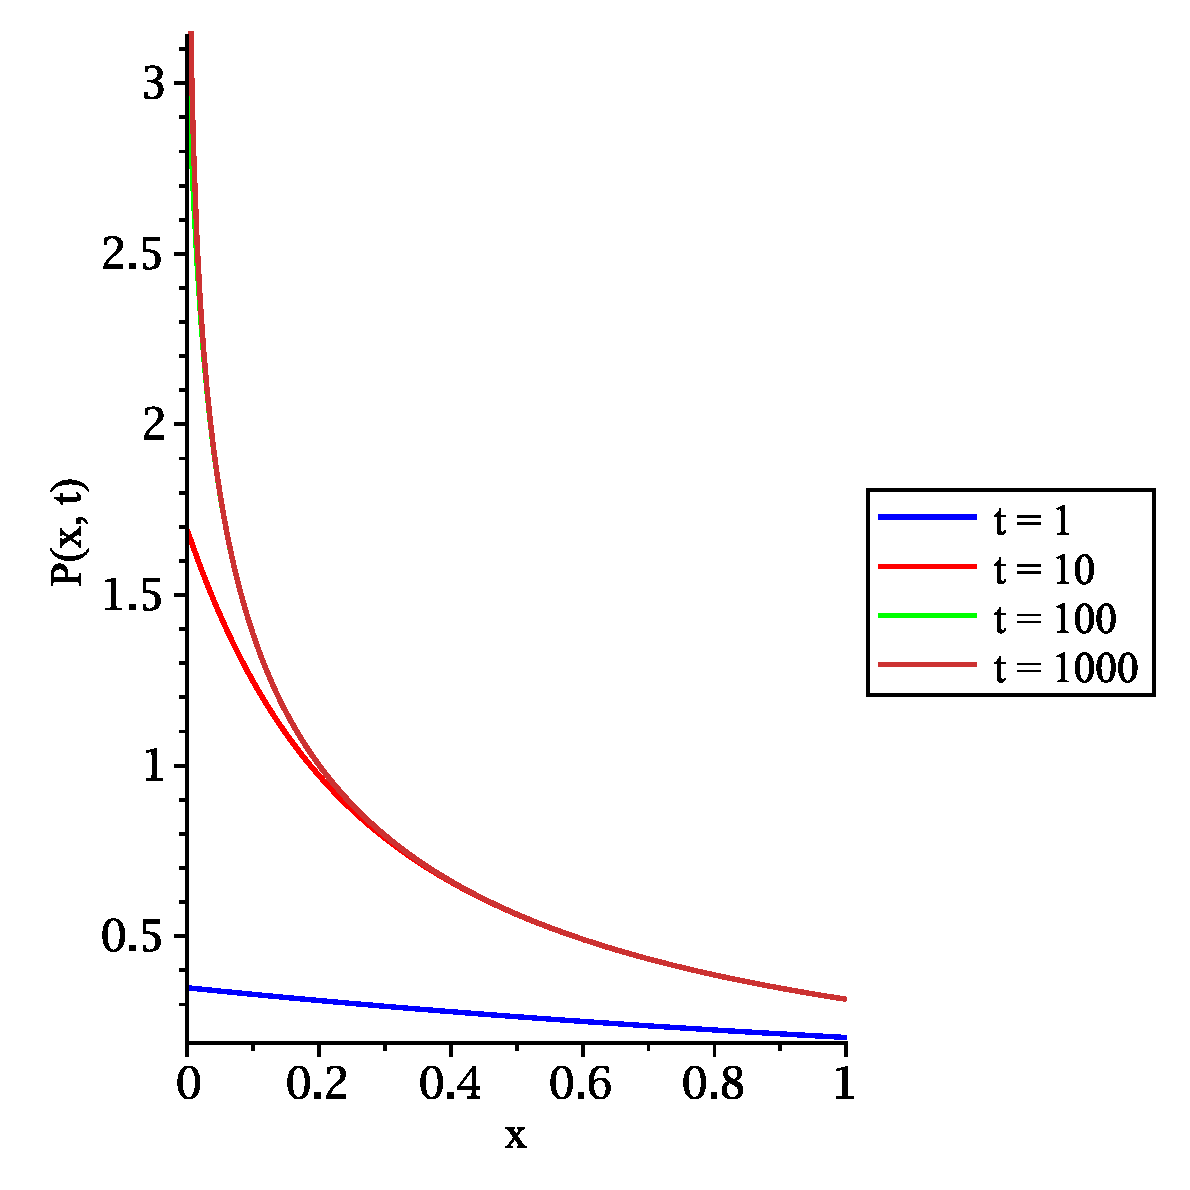
\includegraphics[width=\textwidth]{gap_density_01.eps}
	\caption{The gap density function for $x < 1$}
	\label{fig:gdf1}
\end{figure}\medskip

In figure \ref{fig:gdf1} we see the behaviour of the gap density function for $x < 1$ and 
for a range of values of $t$. As can be seen, as $t$ increases, the density of smaller gaps 
increases sharply, as is to be expected due to the increasing fragmentation, but the density 
of larger gaps within the range becomes more constant, again to be expected because these 
larger gaps are still less than the size of a car, so cannot be occupied, and hence remain 
unchanged. \bigskip

\begin{figure}[h!]
	\centering
%	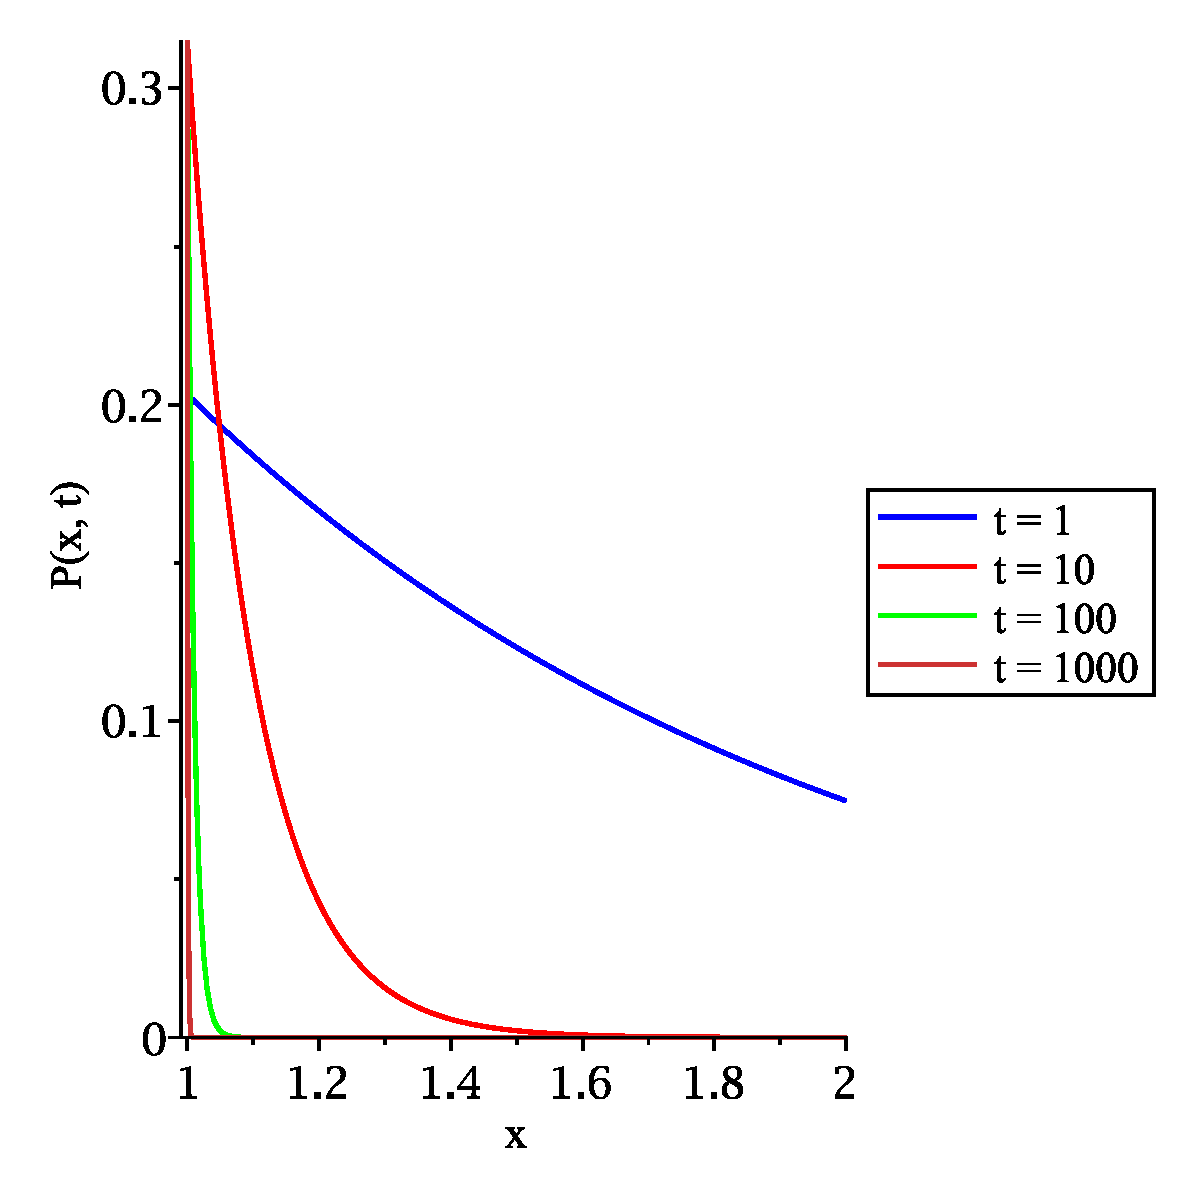
\includegraphics[scale = 0.35]{gap_density_02.eps}
	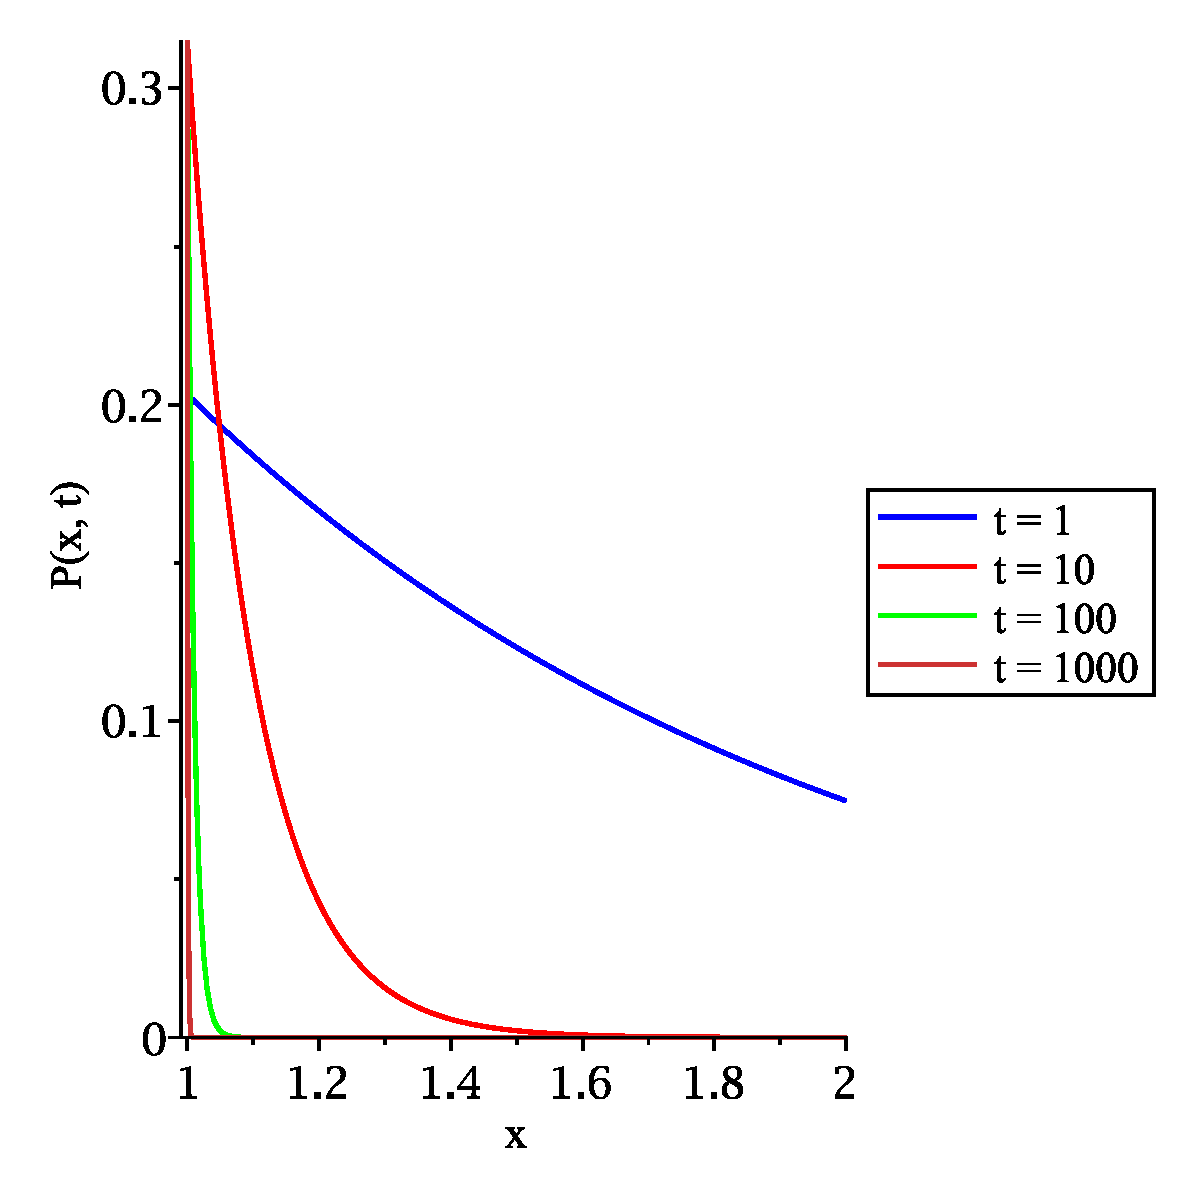
\includegraphics[width=\textwidth]{gap_density_02.eps}
	\caption{The gap density function for $x \geq 1$}
	\label{fig:gdf2}
\end{figure}\medskip

In figure \ref{fig:gdf2} we see the behaviour of the gap density function for $x \geq 1$ and 
for a range of values of $t$. As can be seen, as $t$ increases, the density of smaller gaps 
increases sharply, again as is to be expected due to the increasing fragmentation, but the 
density of larger gaps within the range reduces, again to be expected, because these larger 
gaps are destroyed by cars, and all that remain are gaps not large enough to accommodate cars. \bigskip

\newpage

We next look at the behaviour of the gap density function, $P(x, t)$, as a function of $t$ 
for different values of $x$. \bigskip

\begin{figure}[h!]
	\centering
	%	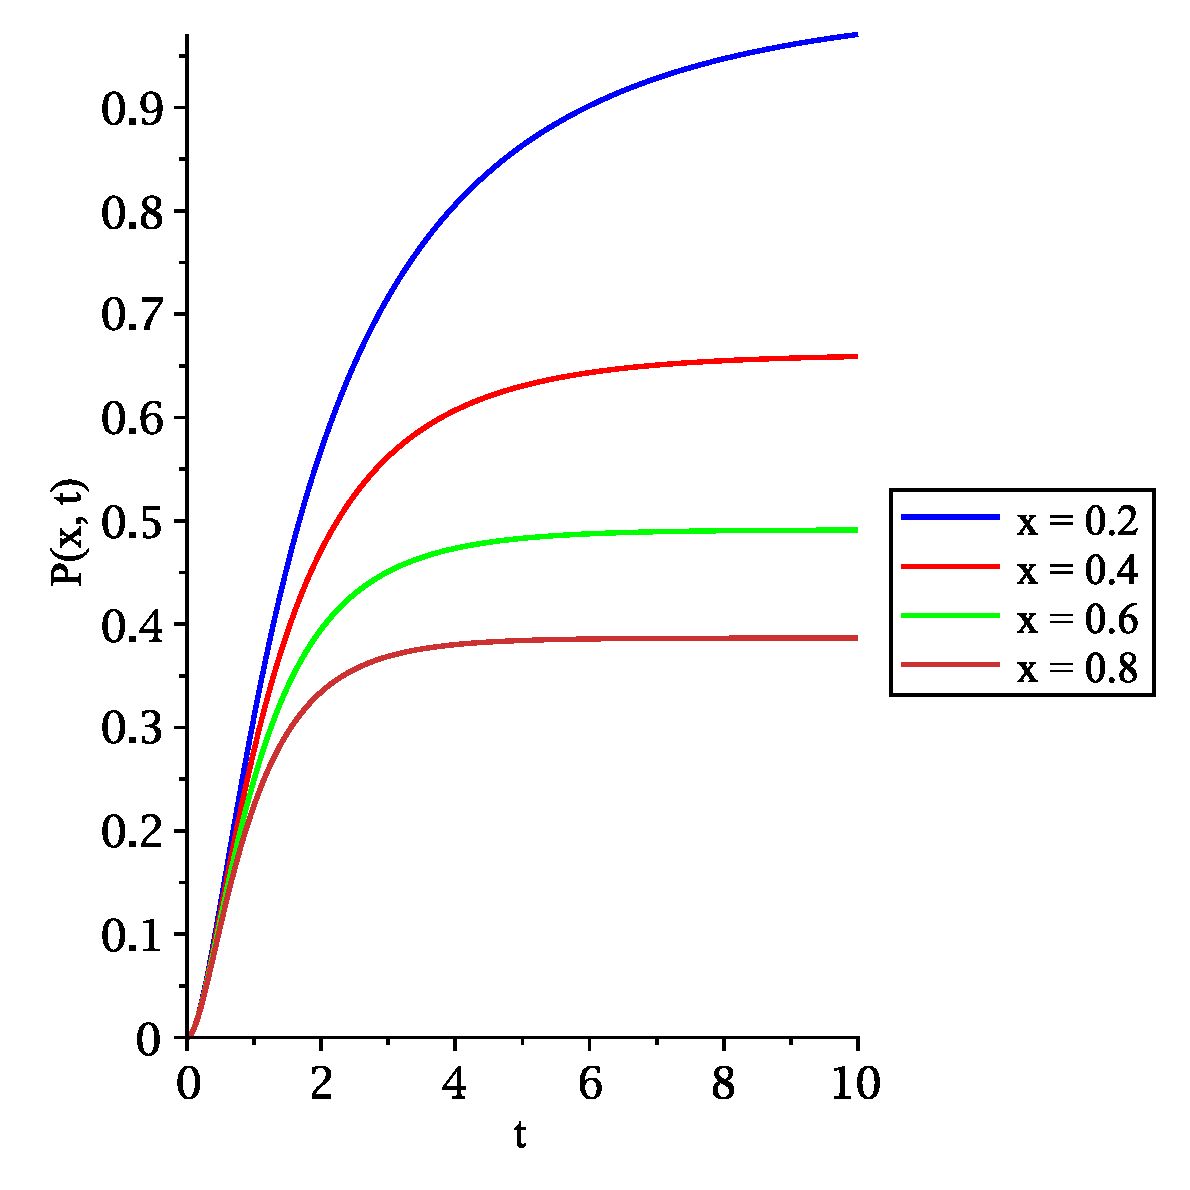
\includegraphics[scale = 0.35]{gap_density_03.eps}
	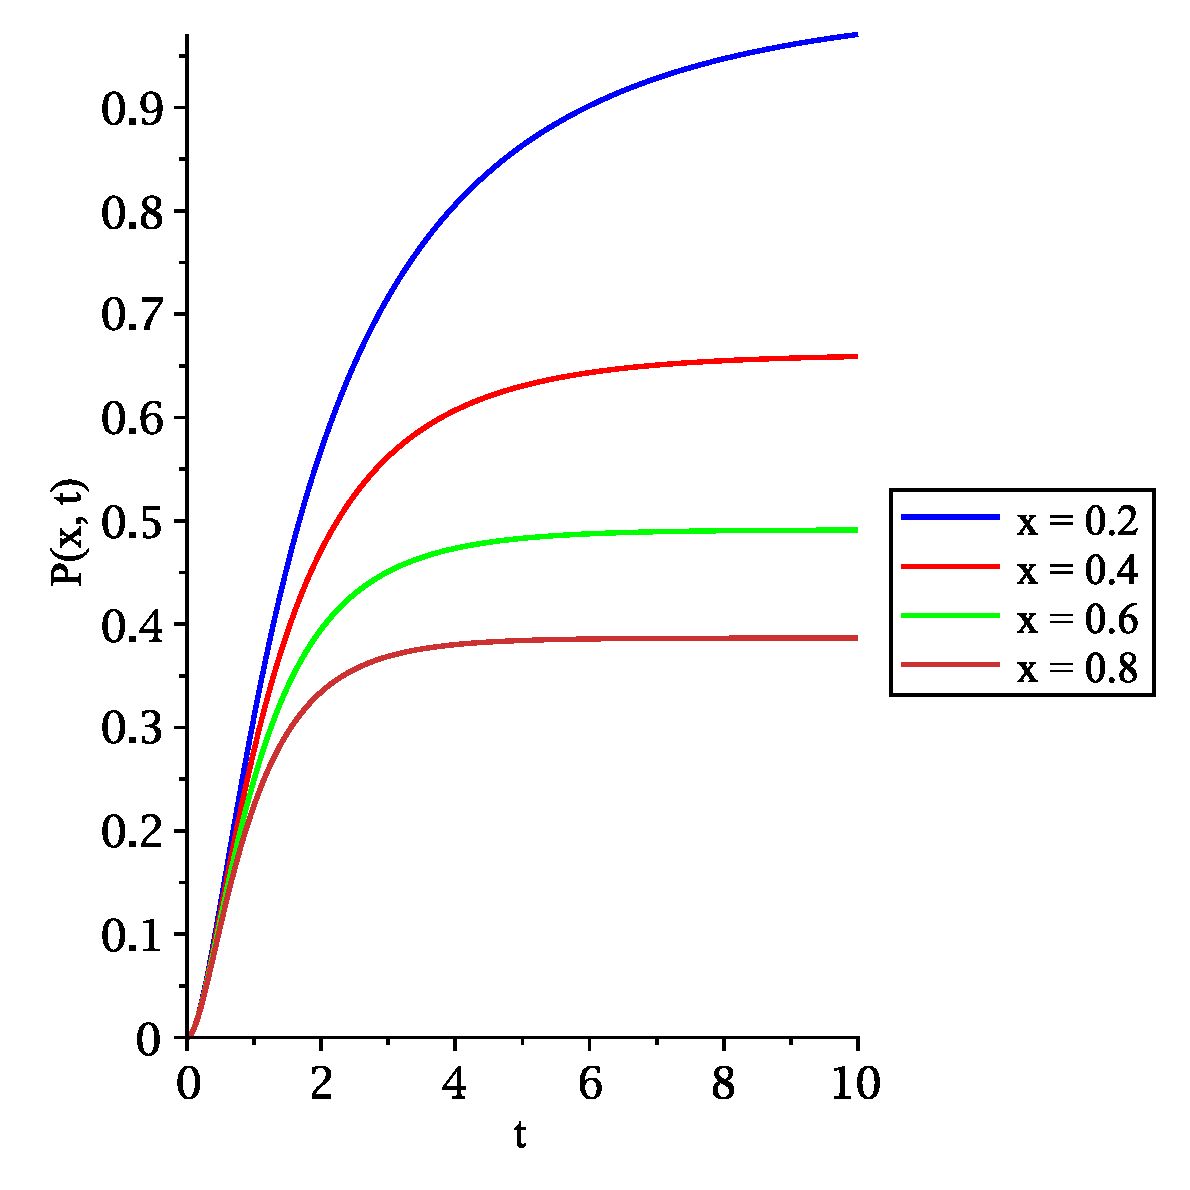
\includegraphics[width=\textwidth]{gap_density_03.eps}
	\caption{The gap density function}
	\label{fig:gdf3}
\end{figure}\medskip

In figure \ref{fig:gdf3} we see the behaviour of the gap density function for a range of 
values of $x < 1$. As can be seen, as $t$ increases, the density of these smaller gaps 
increases to a limit. This is to be expected due to the fact that as the parking process 
continues, eventually gaps, which are less than the size of a car, remain and can never 
be destroyed. \bigskip

\begin{figure}[h!]
	\centering
	%	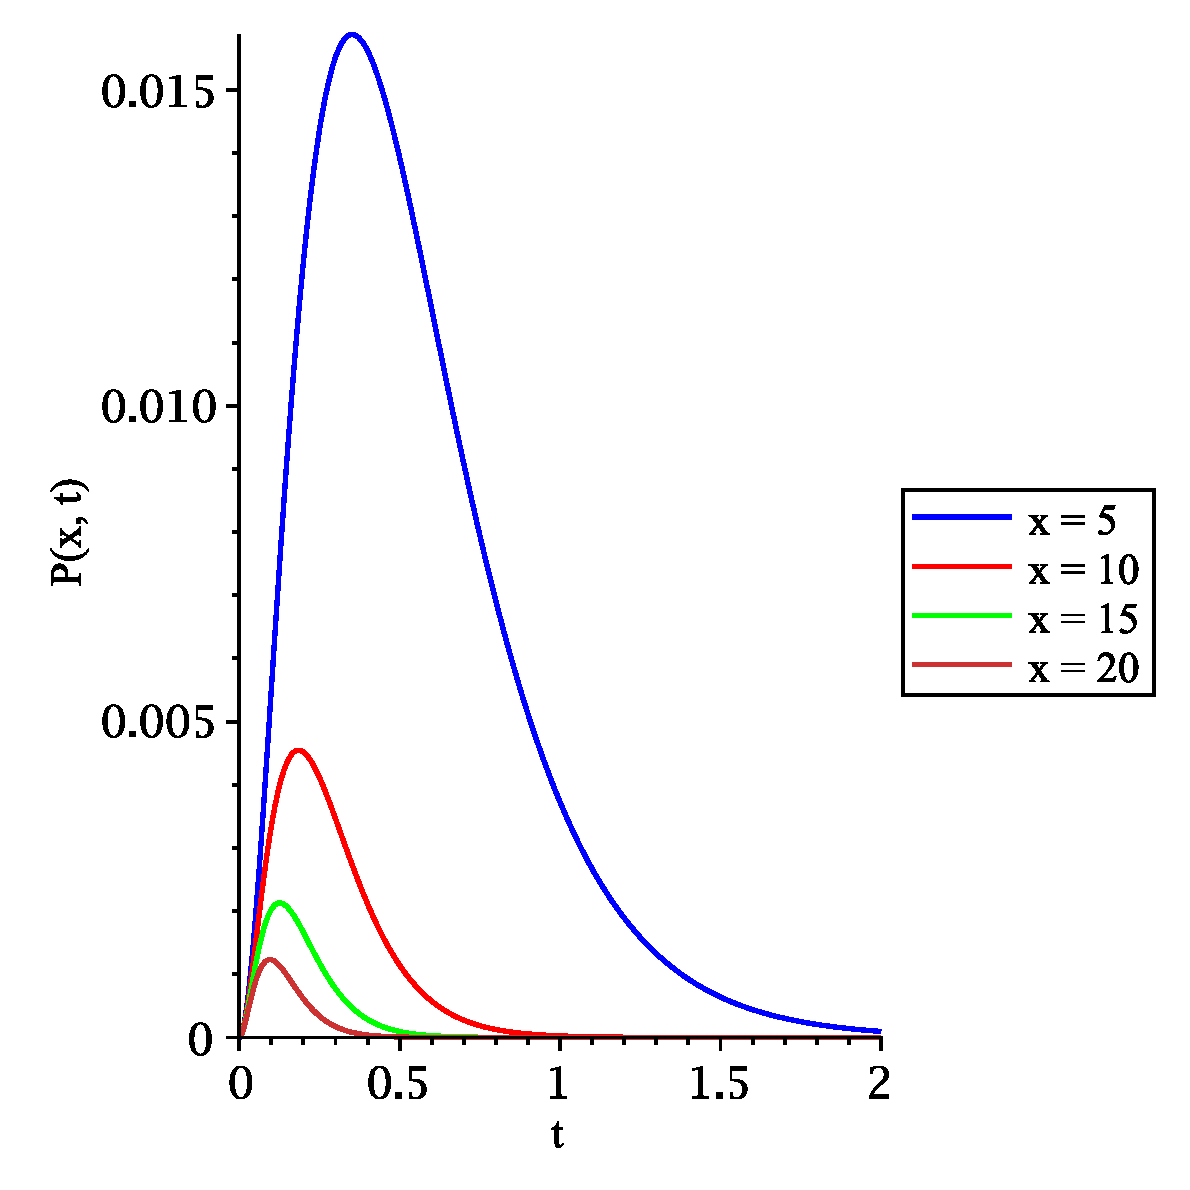
\includegraphics[scale = 0.35]{gap_density_04.eps}
	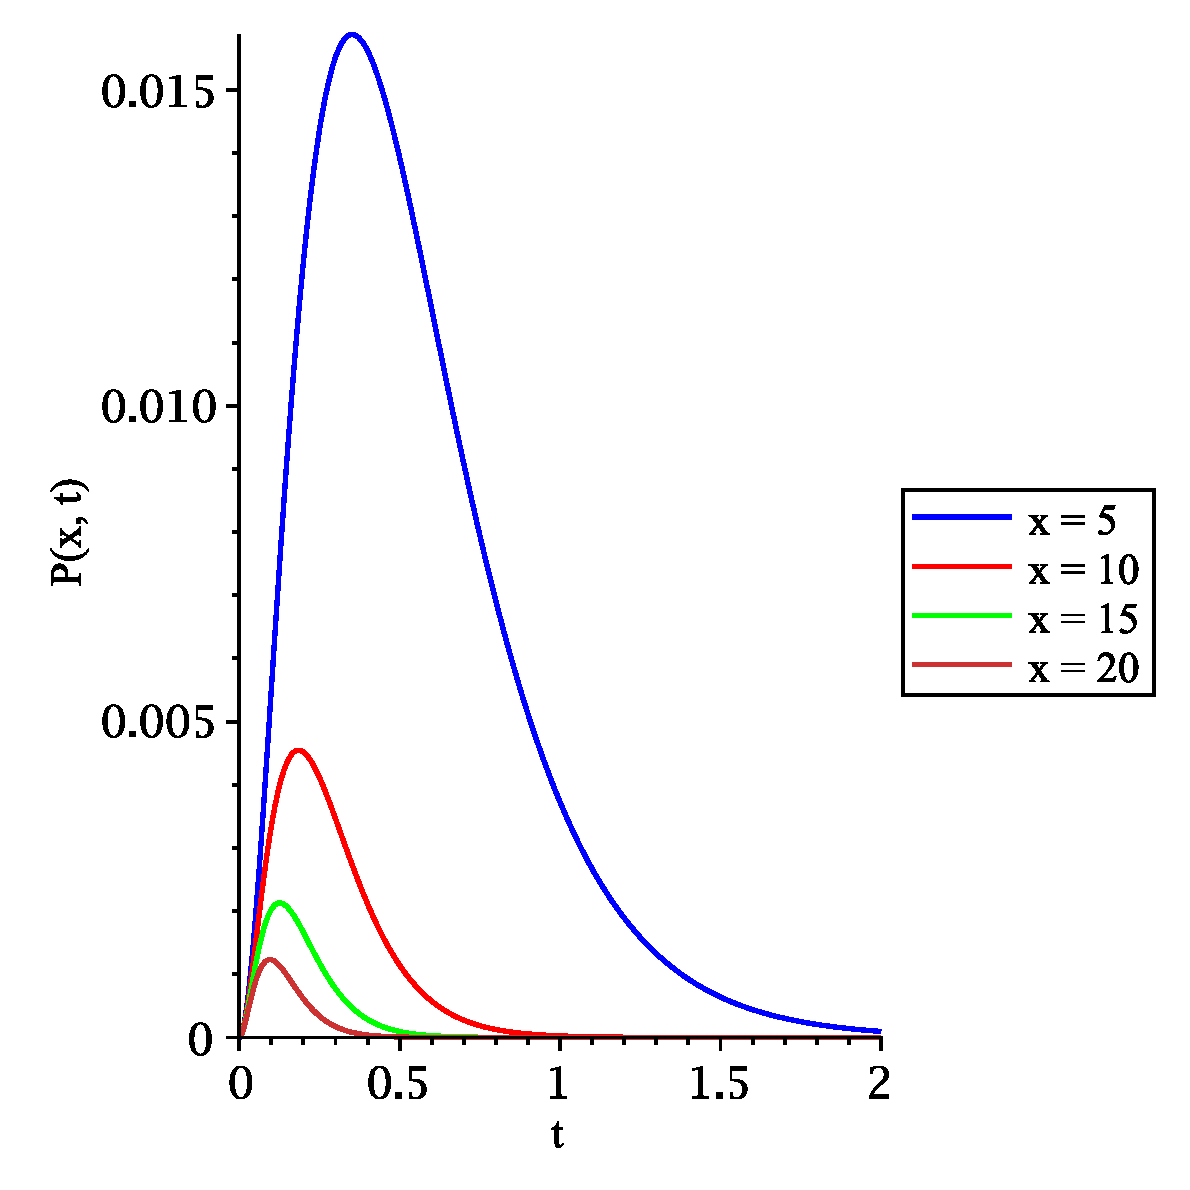
\includegraphics[width=\textwidth]{gap_density_04.eps}
	\caption{The gap density function}
	\label{fig:gdf4}
\end{figure}\medskip

In figure \ref{fig:gdf4} we see the behaviour of the gap density function for a range of 
values of $x \geq 1$. As can be seen, as $t$ increases, the density of these larger gaps 
increases sharply to a maximum, before decreasing, and approaching $0$. This is to be 
expected due to the fact that, as unit cars are initially parked they leave large gaps 
which are eventually destroyed in the parking process. \bigskip











\section{Remarks}

With the kinetic approach we have successfully modelled the process with respect to it's 
time evolution, rather than merely providing a means of evaluating $C_R$. This is a big 
step forward from the previous approaches. \bigskip

It should be noted that the approach of reducing the rate equation to an ODE breaks down 
for finite $L$: \bigskip

\begin{eqnarray*}
			\frac{\partial}{\partial t} (A(t) e^{-(x - 1)t}) & = & -(x - 1) A(t) e^{-(x - 1)t} + 2 \int_{x + 1}^{L} A(t) e^{-(y - 1)t} dy \\\\
	A^{\prime}(t) e^{-(x - 1)t} - (x - 1) A(t) e^{-(x - 1)t} & = & -(x - 1) A(t) e^{-(x - 1)t} + 2 A(t) \left. \frac{e^{-(y - 1)t}}{-t} \right|_{y = x + 1}^{L} \\\\
								 A^{\prime}(t) e^{-(x - 1)t} & = & 2 A(t) \left[ -\frac{e^{-t}}{t} e^{-(L - 2)t} + \frac{e^{-t}}{t} e^{-(x - 1)t} \right] \\\\
															 & = & 2 A(t) \frac{e^{-t}}{t} \left[ e^{-(x - 1)t} - e^{-(L - 2)t} \right]
\end{eqnarray*}\medskip

Hence finite $L$ prevents us from reducing the equation to a more manageable ODE, and it is clear 
that the imposition of $L \to \infty$ is made for mathematical reasons. \bigskip











